\documentclass[10pt,twocolumn]{article}
\usepackage[margin=0.72in]{geometry}
\usepackage{amsmath,amssymb}
\usepackage{booktabs}
\usepackage{graphicx}
\usepackage{hyperref}
\usepackage{microtype}
\usepackage{siunitx}
\usepackage{xcolor}

\hypersetup{
  colorlinks=true,
  linkcolor=blue!60!black,
  citecolor=blue!60!black,
  urlcolor=blue!60!black
}

\title{\textbf{BearingBench: Physics-Informed Order-Domain Inductive Bias, Matryoshka Compression, and Conformal Uncertainty Under Non-Stationary Sensor Shift}}
\author{
  Aryan Hood \\
  \texttt{https://github.com/aryanhood/shm-bearing-dataset}
}
\date{Technical Report}

\begin{document}
\maketitle

\begin{abstract}
Real-world acoustic and vibration edge intelligence faces three coupled failure modes that random i.i.d.\ splits systematically mask: amplitude gain shortcuts across installations, non-stationary spectral smearing under time-varying kinematics, and miscalibrated predictive uncertainty under distribution shift. We present \textsc{BearingBench}, a leak-free, dual-dataset benchmark built over 100 real accelerometer and optical-encoder recordings (40 CWRU 12\,kHz recordings yielding 2,331 windows and 60 uOttawa 200\,kHz speed-varying recordings yielding 699 windows) across 5 random seeds. We study a physics-informed pipeline combining envelope-first 4-band Hilbert Computed Order Tracking (COT), a single-training \textsc{MatryoshkaOrderCNN} supporting elastic prefix slicing ($d \in \{8, 16, 32, 64, 128\}$) and static QDQ INT8 ONNX deployment, leak-free out-of-fold calibration, deep ensembles, and Online Adaptive Conformal Inference (ACI). Under unseen speed regimes on uOttawa, order-domain CNN representation improves accuracy by $+7.61$\,percentage points over a raw time-domain envelope CNN ($96.02\%$ vs.\ $88.41\%$, 95\% bootstrap CI $[+6.61, +8.58]$\,pp, exact McNemar $p < 10^{-10}$), while envelope-first COT beats order-first resampling by $+1.57$\,pp ($92.67\%$ vs.\ $91.10\%$, $p = 1.28 \times 10^{-4}$). Static QDQ INT8 quantization compresses the $d=128$ backbone $3.51\times$ to $35.77\,\text{KB}$ at $92.93\%$ accuracy ($0.1205\,\text{ms}$ p50 CPU latency, zero PyTorch dependency) and sustains $88.04\%$ even at $d=8$ ($19.71\,\text{KB}$). Under unseen CWRU spall diameters ($7/14/21$\,mil), all supervised models collapse ($47.72\%$--$59.63\%$), revealing a fundamental out-of-distribution failure mode where ID-tuned temperature scaling worsens uOttawa OOD ECE ($5.10\% \rightarrow 6.17\%$) while 5-seed ensembles cut OOD ECE to $3.02\%$ and Online ACI recovers $+22.88$\,pp conformal coverage on severe CWRU shift ($50.16\% \rightarrow 73.04\%$).
\end{abstract}

\section{Introduction}
Deployable machine learning for physical and acoustic monitoring must execute within tens of kilobytes on CPU or microcontroller hardware while providing reliable confidence estimates under operating-regime shifts~\cite{das2024timesfm,baur2024hear,narayanswamy2025lsm,zhang2025sensorlm}. Conventional rolling-bearing fault diagnosis benchmarks routinely violate both constraints: window-level random splits leak quasi-periodic samples across recordings~\cite{smith2015cwru,zhao2020deep}, models rely on fixed-speed time-domain spectra that smear when rotational speed varies~\cite{randall2011tutorial,huang2018uottawa}, and classifiers output uncalibrated softmax confidences~\cite{guo2017calibration,ovadia2019trust}.

\textsc{BearingBench} treats vibration fault monitoring as a rigorous benchmark for trustworthy edge time-series learning under realistic distribution shifts. Specifically, we investigate three questions across five random seeds on 100 real laboratory recordings:
\begin{enumerate}
  \item \textbf{Physics inductive bias:} Does extracting structural resonance envelopes across carrier bands \emph{before} angular resampling (envelope-first COT) outperform both time-domain CNNs and order-first resampling on unseen acceleration/deceleration profiles?
  \item \textbf{Precision- and width-elastic edge inference:} Can a single nested \textsc{MatryoshkaOrderCNN}~\cite{kusupati2022matryoshka,nair2025matquant} be sliced at inference time to $d \in \{8, 16, 32, 64, 128\}$ channels and statically INT8-quantized~\cite{jacob2018quantization} into a $20$--$36\,\text{KB}$ ONNX binary with zero PyTorch dependencies?
  \item \textbf{Uncertainty under shift:} When held-out regimes break point predictions---such as unseen spall diameters on CWRU or unseen reversing speed profiles on uOttawa---how do out-of-fold temperature scaling~\cite{guo2017calibration}, 5-seed deep ensembles~\cite{lakshminarayanan2017ensembles}, Split Adaptive Prediction Sets (APS)~\cite{romano2020aps}, and Online ACI~\cite{gibbs2021aci} behave?
\end{enumerate}

\section{Related Work}
\paragraph{Elastic Representations and Quantization.}
Matryoshka Representation Learning (MRL)~\cite{kusupati2022matryoshka} nests coarse-to-fine representations within a single trained vector or channel prefix so deployment hardware can trade width for latency without retraining. This principle underpins elastic Transformer architectures such as MatFormer~\cite{devvrit2024matformer}, patch-elastic FlexiViT~\cite{beyer2023flexivit}, precision-elastic MatQuant~\cite{nair2025matquant}, and compact production checkpoints such as Gemma~3~\cite{gemma2025gemma3}. We adapt MRL channel nesting to a compact 24.8K-parameter 1D convolutional backbone and compose prefix slicing with static Quantize--Dequantize (QDQ) INT8 ONNX export~\cite{jacob2018quantization,nagel2021whitepaper} calibrated strictly inside training folds.

\paragraph{Sensor Foundation Models and Diagnostics.}
Recent time-series and bioacoustic foundation models---including TimesFM~\cite{das2024timesfm}, HeAR~\cite{baur2024hear}, LSM~\cite{narayanswamy2025lsm}, LSM-2~\cite{xu2025lsm2}, and SensorLM~\cite{zhang2025sensorlm}---emphasize robustness to non-stationary, incomplete sensor streams. In mechanical diagnostics, domain tutorials establish envelope analysis~\cite{randall2011tutorial}, cepstrum pre-whitening~\cite{borghesani2013cepstrum}, CWRU pitfalls~\cite{smith2015cwru}, variable-speed benchmarks~\cite{huang2018uottawa}, Paderborn motor-current benchmarks~\cite{lessmeier2016paderborn}, and open-source comparisons~\cite{zhao2020deep}, echoing broader out-of-distribution findings in DomainBed~\cite{gulrajani2021domainbed} and WILDS~\cite{koh2021wilds}.

\paragraph{Calibration and Conformal Risk Control.}
Ovadia et al.~\cite{ovadia2019trust} showed that post-hoc temperature scaling degrades under dataset shift relative to ensembles~\cite{lakshminarayanan2017ensembles}. Selective classification bounds error at fixed coverage~\cite{geifman2017selective}, while split conformal APS~\cite{romano2020aps,angelopoulos2023gentle}, training-time conformal objectives~\cite{stutz2022conftr}, and Conformal Risk Control~\cite{angelopoulos2024crc} certify prediction sets under exchangeability. For streaming regime shift, Gibbs and Cand\`es' Adaptive Conformal Inference (ACI)~\cite{gibbs2021aci} dynamically updates $\alpha_t$ to restore long-run target coverage.

\section{Methodology}
\subsection{Order-Domain Physics Inductive Bias}
Under time-varying shaft speed $\omega(t)$, bearing fault impacts occur at fixed kinematic shaft orders rather than fixed frequencies in Hz. Given a 200\,kHz accelerometer stream and a 1024-PPR optical encoder trace (sampled per Schmitt-trigger rising edge with sub-sample linear interpolation), naive \emph{order-first} COT resamples raw vibration before bandpass filtering, shifting structural resonance frequencies as speed changes. Our \emph{envelope-first} COT (1) bandpasses the time-domain signal into four structural carrier bands ($[0.5\text{--}5, 5\text{--}15, 15\text{--}35, 35\text{--}65]$\,kHz), (2) extracts the Hilbert analytic amplitude and squares it in time, (3) resamples each nonnegative band envelope onto uniform shaft-angle grids ($\Delta\theta = 2\pi / 1024$\,rad) via PCHIP/cubic interpolation over 2-revolution windows, and (4) computes the gain-invariant median-normalized FFT Squared Envelope Spectrum (SES) yielding an input tensor $x \in \mathbb{R}^{4 \times 400}$. Figure~\ref{fig:physics} illustrates this de-smearing on uOttawa \texttt{O-C-1}.

\begin{figure*}[t]
  \centering
  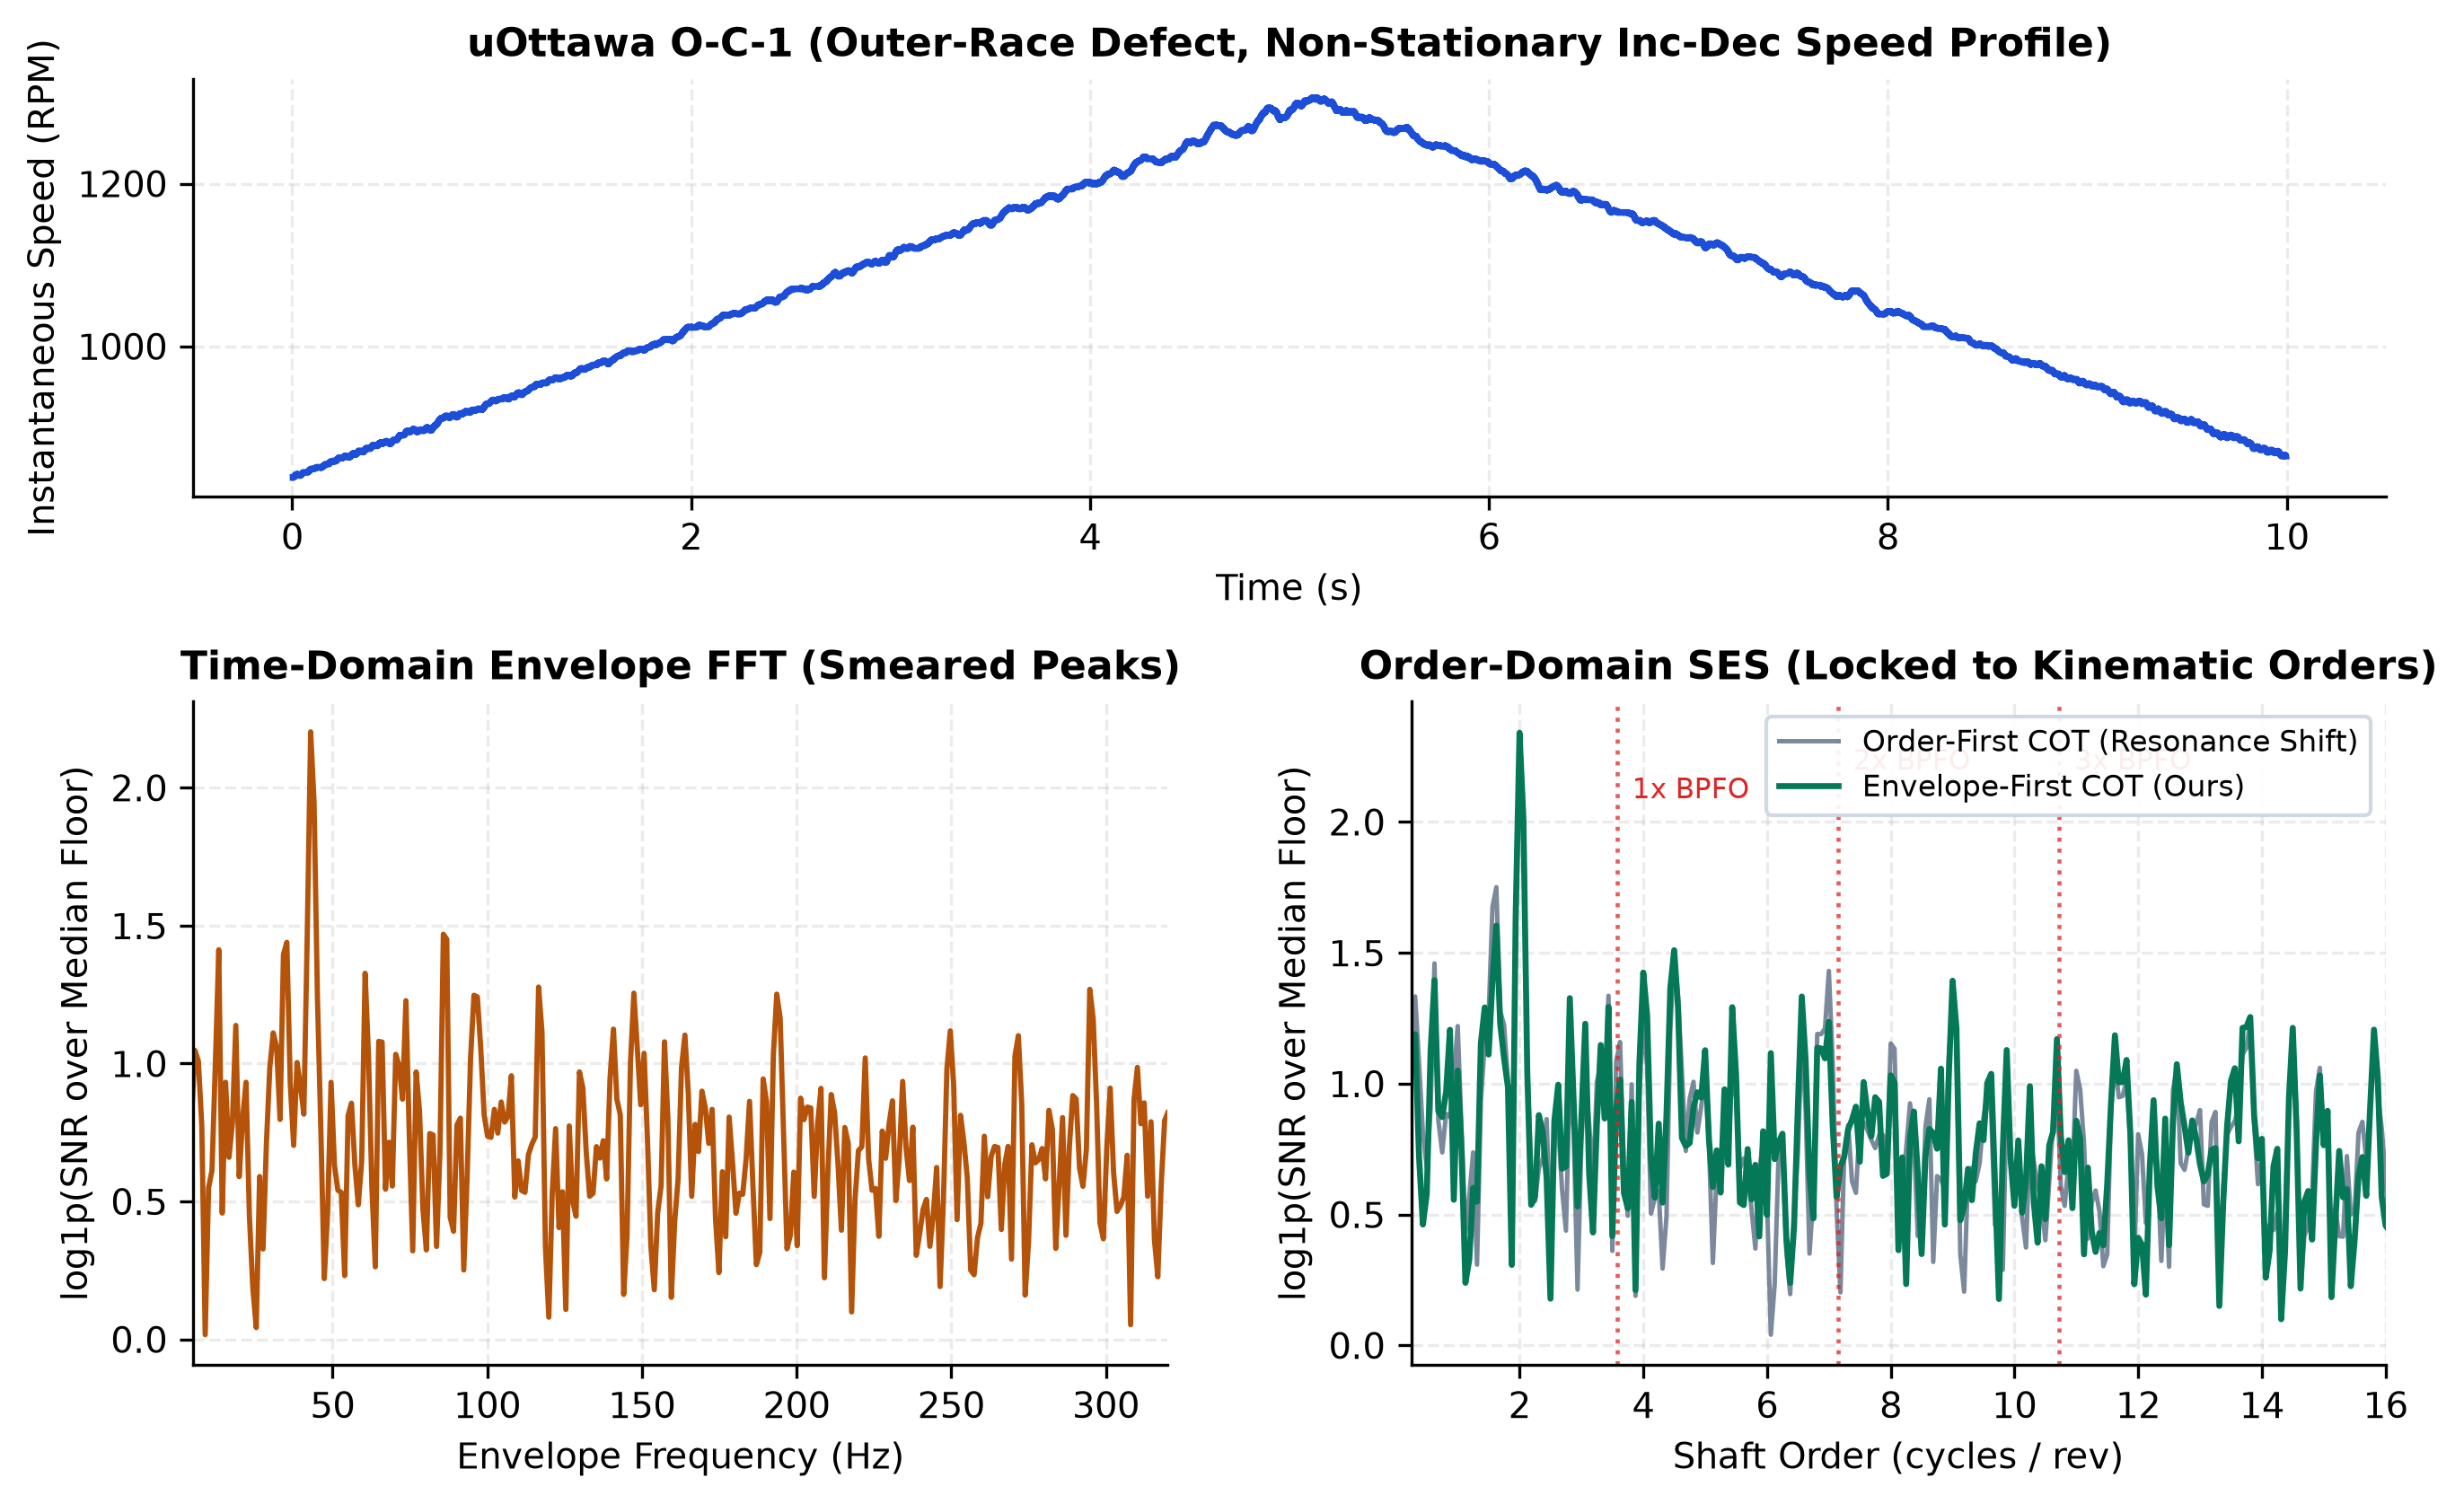
\includegraphics[width=0.96\textwidth]{../assets/fig2_physics_order_vs_time.png}
  \caption{Real uOttawa \texttt{O-C-1} recording (inc--dec speed $840 \leftrightarrow 1300$\,RPM): time-domain envelope FFT smears outer-race fault harmonics, whereas envelope-first COT locks SNR peaks to kinematic shaft orders ($k \times \text{BPFO}$).}
  \label{fig:physics}
\end{figure*}

\subsection{Elastic \textsc{MatryoshkaOrderCNN} and Static INT8}
\textsc{MatryoshkaOrderCNN} applies three 1D convolutional blocks ($C \in \{4 \rightarrow 32 \rightarrow 64 \rightarrow 128\}$) followed by global average pooling and a linear head $W \in \mathbb{R}^{K \times 128}$. Let $\mathcal{D} = \{8, 16, 32, 64, 128\}$. During training, we optimize the equally weighted nested cross-entropy loss:
\begin{equation}
  \mathcal{L}_{\text{MRL}}(x, y) = \frac{1}{|\mathcal{D}|} \sum_{d \in \mathcal{D}} \text{CE}\!\left(W_{:, :d}\, z(x)_{:d} + b,\, y\right).
\end{equation}
For hardware deployment at budget $d \in \mathcal{D}$, \textsc{SlicedMatryoshkaCNN} structurally slices the final pointwise convolution kernels and linear head down to $d$ channels (producing physical parameter and FLOP savings, not zero-masking), exports opset-18 ONNX graphs, and applies static QDQ INT8 quantization calibrated exclusively on proper-training windows. Inference runs via \textsc{EdgeClassifier} on single-thread CPU ONNX Runtime with zero PyTorch or scikit-learn dependencies.

\subsection{Calibration, Conformal Prediction, and Safety Supervisor}
For every protocol and seed, we fit scalar Temperature Scaling via leak-free 2-fold recording-grouped out-of-fold (OOF) logits strictly inside the training mask. We compare OOF Temperature Scaling and 5-seed ensembles on ECE, Brier score, NLL, and selective risk--coverage (AURC). At target coverage $1-\alpha = 0.90$, we compare static Split APS~\cite{romano2020aps} calibrated on proper-train OOF probabilities against chronological Online ACI~\cite{gibbs2021aci} ($\gamma = 0.05$, $\alpha_{t+1} = \alpha_t + \gamma(\alpha - \text{err}_t)$). When $|C(x_t)| > 1$, when calibrated severe fault probability crosses confirmation hysteresis ($3$-of-$4$ windows), or when a sensor fault is detected (clipping/dropout audit), \textsc{SupervisoryController} triggers slew-limited \texttt{DERATE} or \texttt{SAFE\_STOP} commands.

\section{Experimental Setup}
\paragraph{Datasets and Leak-Free Protocols.}
We evaluate exclusively on real public \texttt{.mat} recordings (five seeds $\{7, 19, 42, 73, 101\}$):
\begin{itemize}
  \item \textbf{CWRU (40 recordings, 2,331 windows, 4 classes):} \texttt{random\_window} (5-fold window split, leakage control), \texttt{unseen\_load} (leave-one-HP-out $0..3$\,HP), and \texttt{unseen\_fault\_size} (leave-one-spall-diameter-out $7/14/21$\,mil with load-matched normals).
  \item \textbf{uOttawa (60 recordings, 699 windows, 5 classes):} \texttt{random\_window}, \texttt{unseen\_trial} (3-fold grouped by trial $1..3$), and \texttt{unseen\_speed\_profile} (train monotonic $A/B \leftrightarrow$ test reversing $C/D$).
\end{itemize}

\begin{table*}[t]
\centering
\small
\caption{Zero-label unsupervised drift vs.\ ISO~20816-3 and 5-seed supervised accuracy (mean $\pm$ std \%) across CWRU and uOttawa protocols.}
\begin{tabular}{llccc}
\toprule
Dataset & Model / Representation & \texttt{random\_window} & Unseen Load / Trial & Unseen Size / Speed \\
\midrule
CWRU (4-cls) & Gain-Sensitive 16-d MLP & $99.98 \pm 0.02$ & $99.90 \pm 0.04$ & $59.29 \pm 2.90$ \\
CWRU (4-cls) & Gain-Invariant 27-d RF & $96.20 \pm 0.12$ & $94.83 \pm 0.10$ & $42.32 \pm 0.83$ \\
CWRU (4-cls) & Env 1D-CNN & $99.00 \pm 0.08$ & $95.44 \pm 0.56$ & $59.63 \pm 1.22$ \\
CWRU (4-cls) & MRL Env 1D-CNN ($d=128$) & $98.14 \pm 0.12$ & $95.29 \pm 0.15$ & $47.72 \pm 2.47$ \\
\midrule
uOttawa (5-cls) & Time-Env RF & $91.59 \pm 0.50$ & $91.22 \pm 0.45$ & $86.04 \pm 0.55$ \\
uOttawa (5-cls) & Time-Env 1D-CNN & $94.28 \pm 0.43$ & $93.05 \pm 0.95$ & $88.41 \pm 1.19$ \\
uOttawa (5-cls) & Order-Physics RF & $97.42 \pm 0.10$ & $96.97 \pm 0.12$ & $93.25 \pm 0.16$ \\
uOttawa (5-cls) & Order 1D-CNN & $\mathbf{99.00 \pm 0.27}$ & $\mathbf{98.46 \pm 0.21}$ & $\mathbf{96.02 \pm 0.52}$ \\
uOttawa (5-cls) & Order-MRL 1D-CNN ($d=128$) & $96.60 \pm 0.59$ & $95.36 \pm 0.66$ & $92.67 \pm 0.83$ \\
\bottomrule
\end{tabular}
\label{tab:main}
\end{table*}

\section{Results and Ablations}
\subsection{Zero-Label Baselines vs.\ ISO~20816-3 and Main Benchmark}
On CWRU, ISO~20816-3 velocity RMS ($10$--$1000$\,Hz) assigns $40/40$ recordings to healthy Zone~A ($36/36$ faults masked) because structural impacts excite kHz carriers with modest low-frequency RMS velocity. In contrast, our zero-label Median/MAD carrier-band drift score achieves $1.00$ AUROC / $1.00$ AUPRC on CWRU (healthy max $15.94$, fault min $44.50$) and $0.9097$ AUROC / $0.9739$ AUPRC on uOttawa unseen speed profiles $C/D$.

Table~\ref{tab:main} and Figure~\ref{fig:bench} summarize all supervised protocols. On uOttawa \texttt{unseen\_speed\_profile}, switching from time-domain to order-domain 1D-CNN yields $+7.61$\,pp ($96.02\%$ vs.\ $88.41\%$; pooled paired bootstrap 95\% CI $[+6.61, +8.58]$\,pp, exact McNemar $305$ vs.\ $39$, $p < 10^{-10}$). Training \textsc{Order-MRL} with uniform nested supervision retains $92.67\%$ ($p = 0.220$ vs.\ 27-feature physics RF), trading $3.35$\,pp top-width accuracy for prefix elasticity.

\begin{figure*}[t]
  \centering
  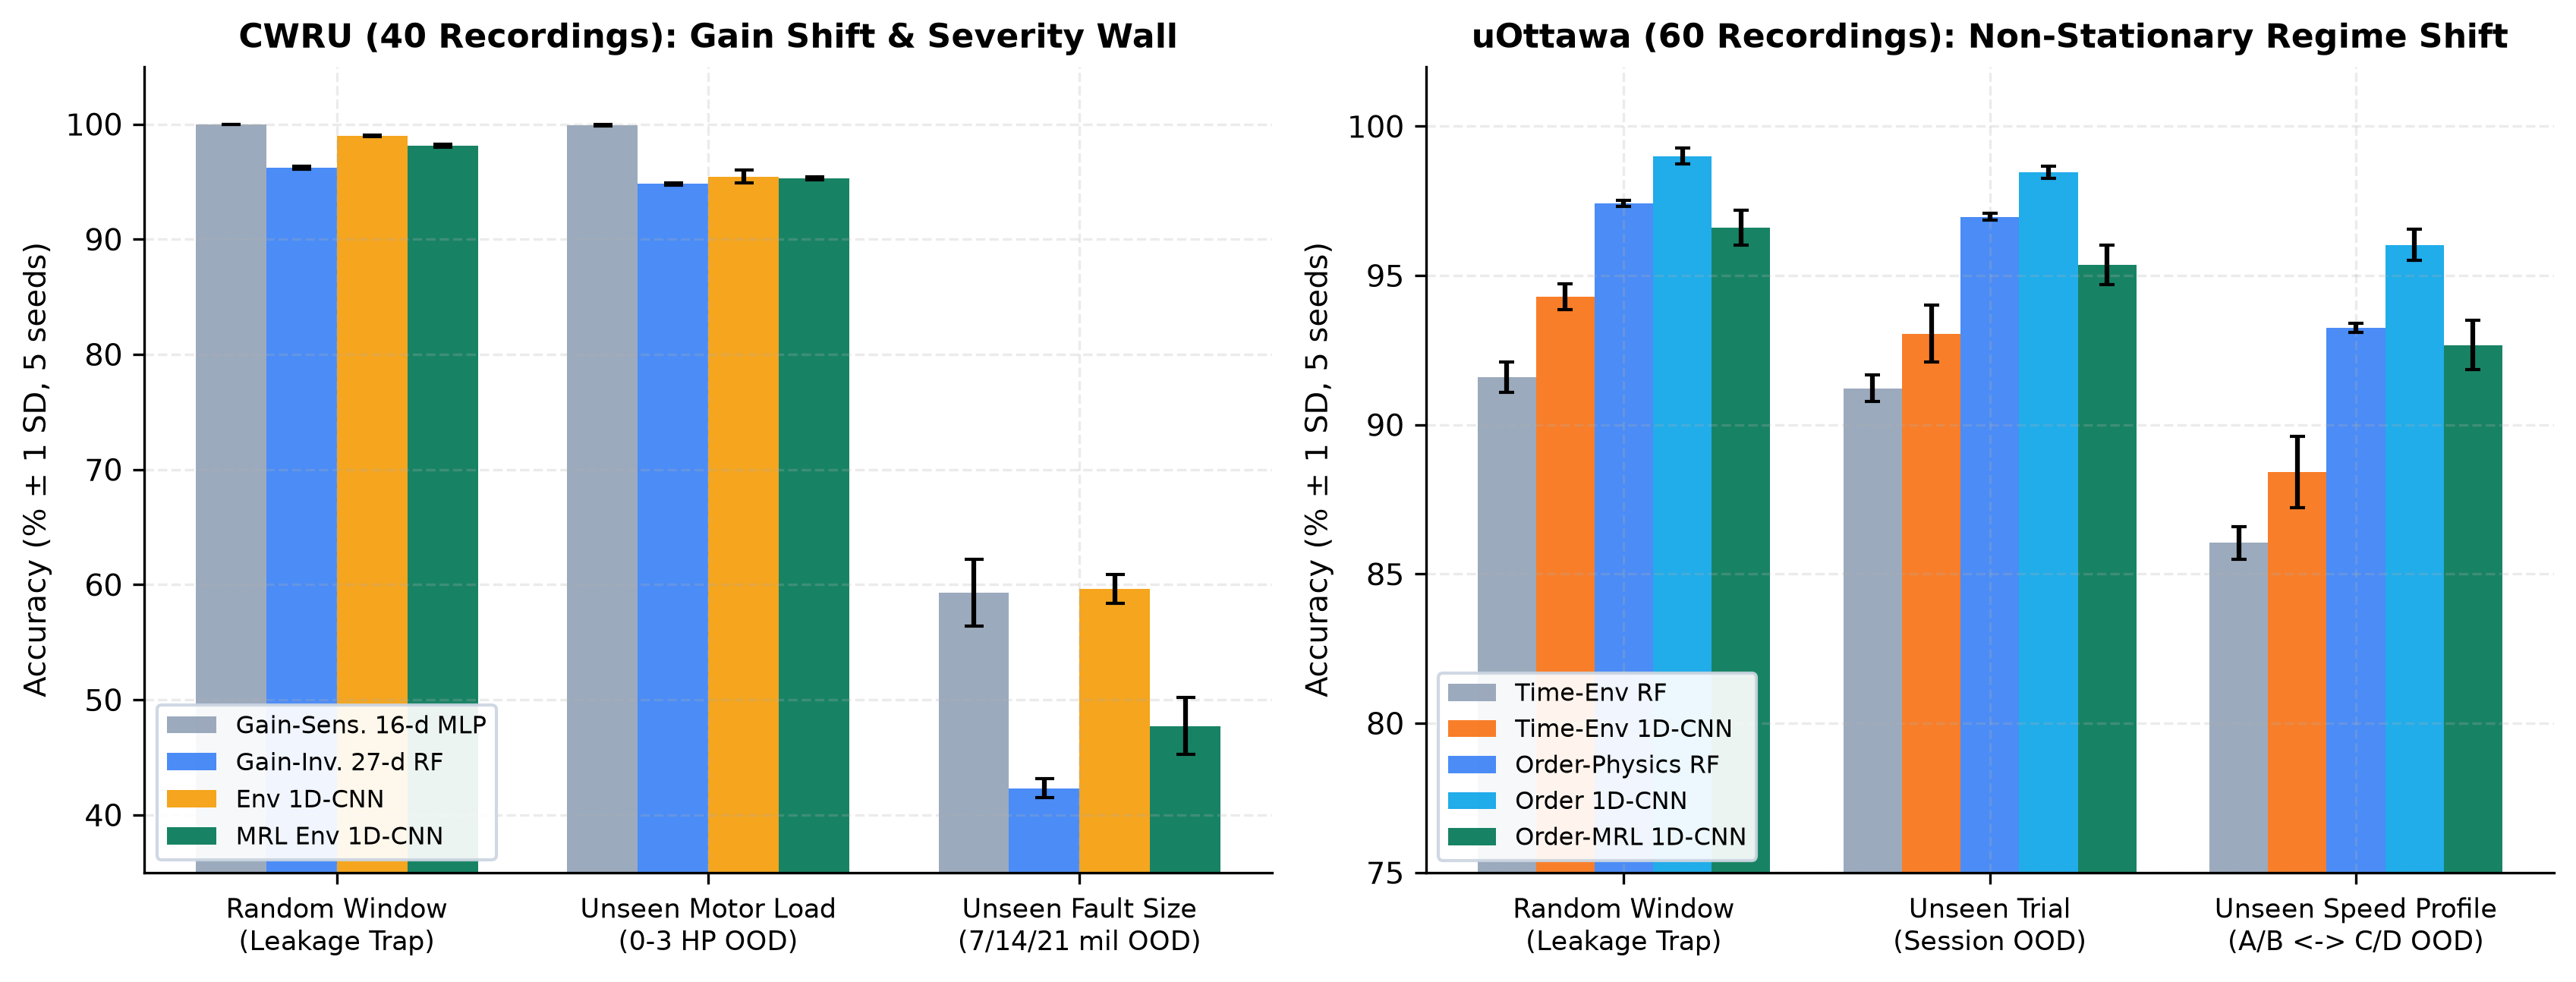
\includegraphics[width=0.96\textwidth]{../assets/fig3_dual_dataset_benchmark.png}
  \caption{5-seed accuracy ($\pm 1$\,SD) across CWRU (gain shift and unseen fault severity wall) and uOttawa (time-domain smearing vs.\ order-domain stability).}
  \label{fig:bench}
\end{figure*}

\subsection{Factorial Signal-Processing and Tachometer Ablations}
Varying one pipeline factor at a time across 5 seeds on uOttawa \texttt{unseen\_speed\_profile} confirms every physical design choice (Figure~\ref{fig:pareto}, left):
\begin{itemize}
  \item \textbf{Envelope-first vs.\ order-first COT:} $92.67 \pm 0.83\%$ vs.\ $91.10 \pm 0.33\%$ ($+1.57$\,pp overall, 95\% CI $[+0.80, +2.35]$\,pp, McNemar $128$ vs.\ $73$, $p = 0.000128$; ball fault recall $82.61\%$ vs.\ $78.55\%$).
  \item \textbf{Cepstrum pre-whitening (CPW):} Slightly reduces accuracy to $92.33 \pm 0.51\%$ (ball recall $80.44\%$), showing flattening log-spectra can attenuate diagnostic sidebands under non-stationary SNR.
  \item \textbf{Single-band collapse:} Restricting to one band drops accuracy to $90.10\%$ ($0.5$--$5$\,kHz), $81.14\%$ ($5$--$15$\,kHz), and $65.49\%$ ($15$--$35$\,kHz), confirming multi-band fusion is essential.
  \item \textbf{Encoder resolution \& edge jitter:} Downsampling from $1024$\,PPR to $256$, $64$, and $32$\,PPR plus adding $2\%$ simulated edge jitter yields $92.64\%$--$92.70\%$ accuracy because even $32$\,PPR gives $64$ smoothed edges per 2-revolution window.
\end{itemize}

\begin{figure*}[t]
  \centering
  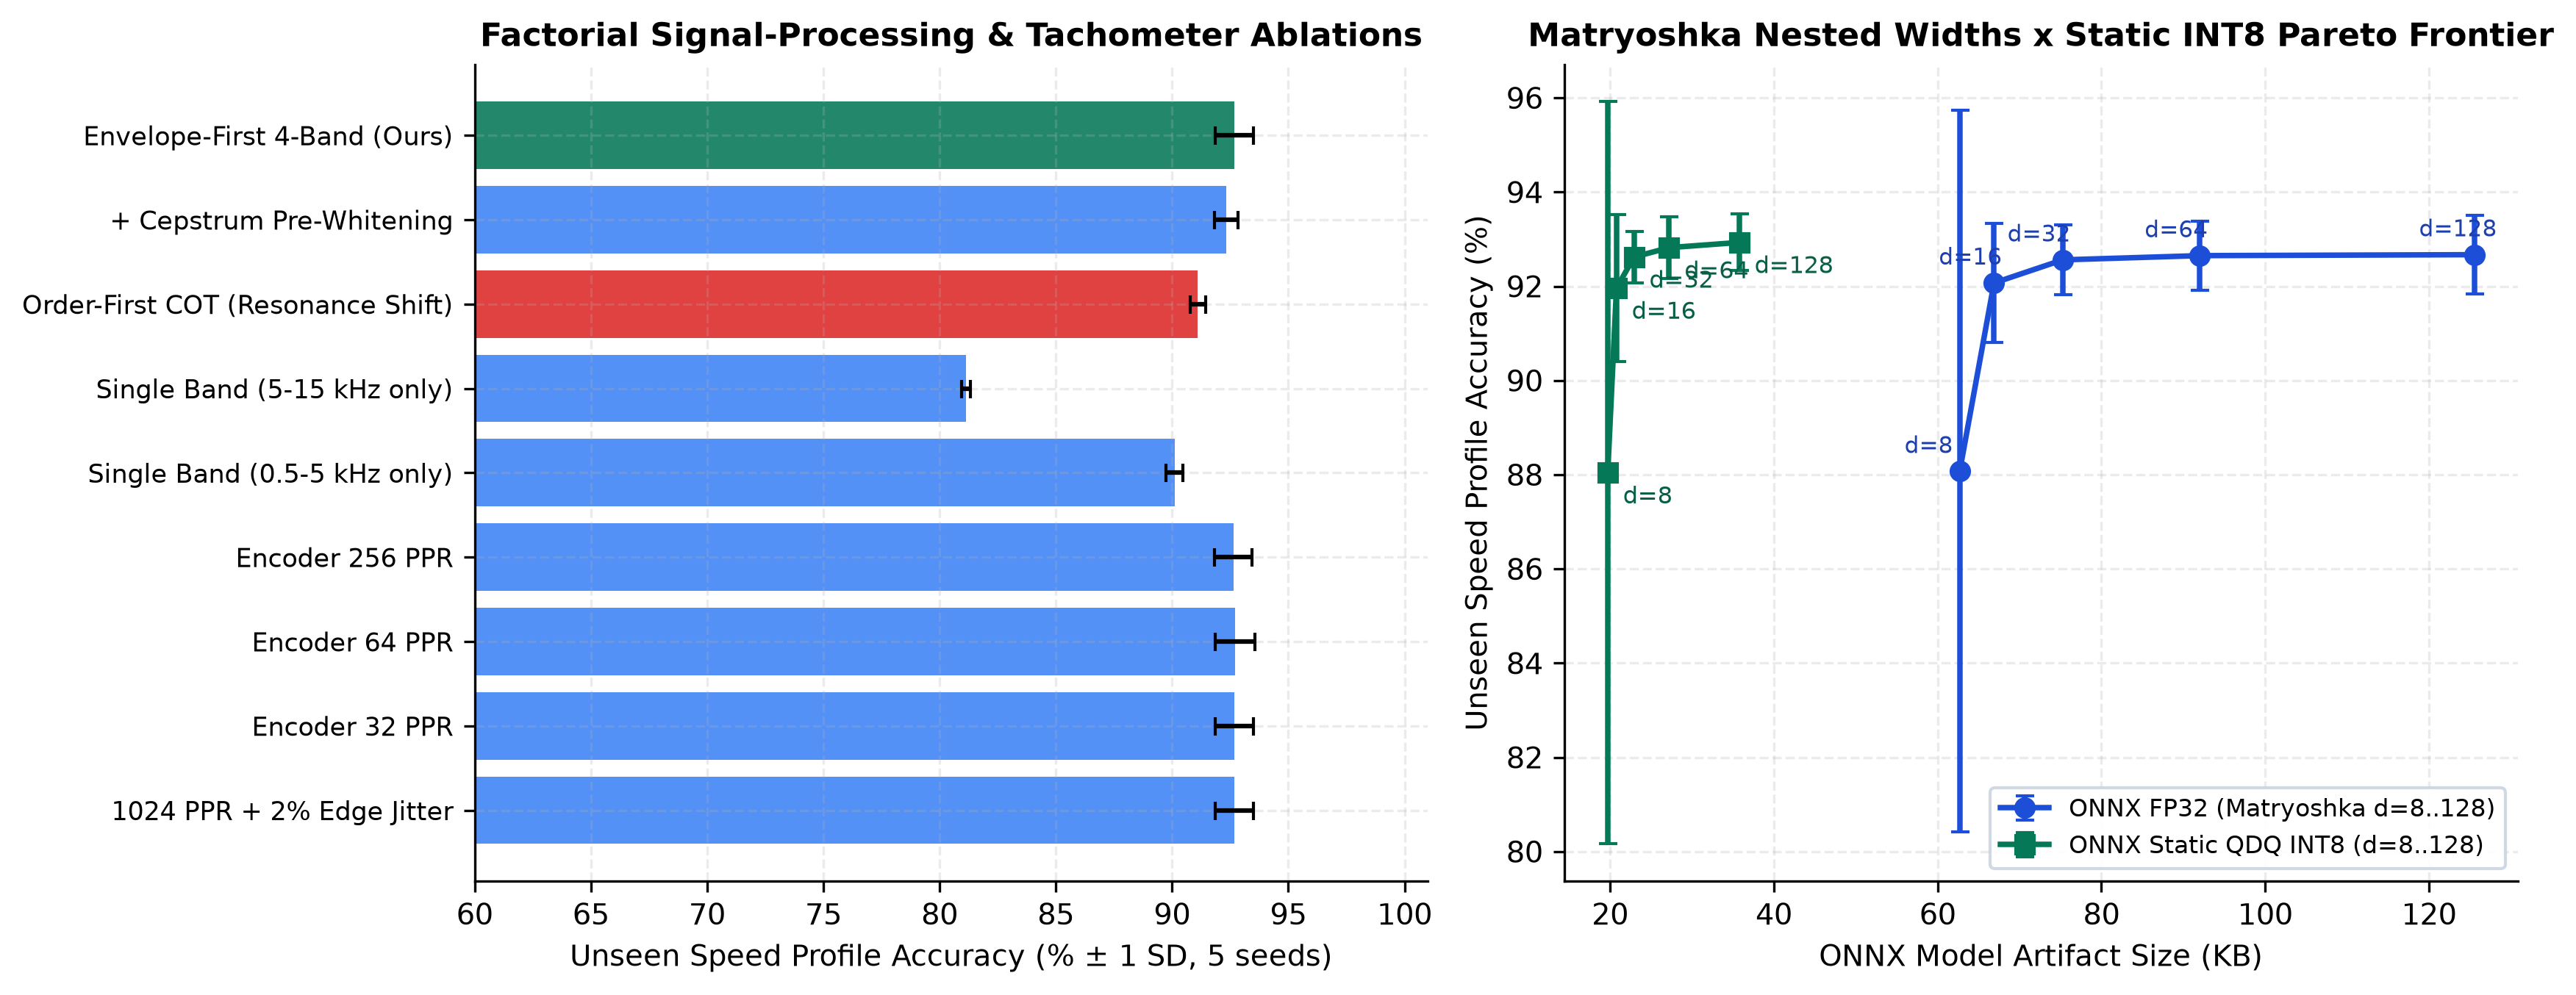
\includegraphics[width=0.96\textwidth]{../assets/fig4_ablations_and_mrl_pareto.png}
  \caption{Left: 5-seed factorial signal-processing and tachometer ablations on \texttt{unseen\_speed\_profile}. Right: Matryoshka width vs.\ Static QDQ INT8 Pareto frontier ($19.71\,\text{KB}$--$125.52\,\text{KB}$).}
  \label{fig:pareto}
\end{figure*}

\subsection{Matryoshka Elastic Compression and Static QDQ INT8 Pareto}
Table~\ref{tab:pareto} and Figure~\ref{fig:pareto} (right) report the full accuracy--size--latency frontier across $d \in \{8, 16, 32, 64, 128\}$. Parity between PyTorch and FP32 ONNX holds to $1.62 \times 10^{-5}$ max logit difference. Static QDQ INT8 quantization compresses artifacts by $3.2$--$3.5\times$ while preserving or slightly improving test accuracy at $d \ge 32$ ($92.93\%$ INT8 vs.\ $92.67\%$ FP32 at $d=128$, $35.77\,\text{KB}$, $0.1205\,\text{ms}$ p50 CPU latency; $91.96\%$ at $d=16$ in $20.78\,\text{KB}$). Notably, $d=32$ INT8 achieves both $92.62 \pm 0.55\%$ accuracy and the lowest OOD ECE ($0.0265$) of any sliced width.

\begin{table}[t]
\centering
\scriptsize
\caption{Matryoshka ONNX FP32 vs.\ Static QDQ INT8 on uOttawa \texttt{unseen\_speed\_profile} (5 seeds).}
\begin{tabular}{rccccc}
\toprule
$d$ & Prec. & Acc ($\pm$SD)\% & Size (KB) & p50 (ms) & ECE \\
\midrule
8 & FP32 & $88.07 \pm 7.66$ & 62.69 & 0.1549 & 0.1777 \\
8 & INT8 & $88.04 \pm 7.88$ & \textbf{19.71} & \textbf{0.1045} & 0.1802 \\
16 & FP32 & $92.07 \pm 1.26$ & 66.88 & 0.4440 & 0.0556 \\
16 & INT8 & $91.96 \pm 1.56$ & 20.78 & 0.1908 & 0.0525 \\
32 & FP32 & $92.56 \pm 0.74$ & 75.26 & 0.2236 & 0.0260 \\
32 & INT8 & $92.62 \pm 0.55$ & 22.92 & 0.2238 & \textbf{0.0265} \\
64 & FP32 & $92.65 \pm 0.73$ & 92.01 & 0.1143 & 0.0432 \\
64 & INT8 & $92.82 \pm 0.66$ & 27.21 & 0.0763 & 0.0425 \\
128 & FP32 & $92.67 \pm 0.83$ & 125.52 & 0.1800 & 0.0510 \\
128 & INT8 & $\mathbf{92.93 \pm 0.60}$ & 35.77 & 0.1205 & 0.0514 \\
\bottomrule
\end{tabular}
\label{tab:pareto}
\end{table}

\subsection{Calibration, Conformal Sets, and Closed-Loop Replay}
Consistent with Ovadia et al.~\cite{ovadia2019trust}, uOttawa shift from \texttt{random\_window} to \texttt{unseen\_speed\_profile} doubles raw single-model ECE ($2.63\% \rightarrow 5.10\%$), and ID-tuned OOF temperature scaling worsens OOD ECE ($6.17\%$, NLL $0.7656$) while 5-seed ensembling reduces OOD ECE to $3.02\%$ (NLL $0.3108$, accuracy $93.85\%$, Figure~\ref{fig:cal}). Across protocols, Online ACI maintains adaptive target coverage ($93.93\%$ on \texttt{unseen\_speed\_profile}, $96.25\%$ on \texttt{unseen\_trial}) and rescues catastrophic Split APS under-coverage on CWRU \texttt{unseen\_fault\_size} by $+22.88$\,pp ($50.16\% \rightarrow 73.04\%$, Table~\ref{tab:uq}).

On the continuous Trial-3 replay (\texttt{H-C-3} healthy followed by \texttt{C-C-3} combined fault, Figure~\ref{fig:replay}), the $35.77\,\text{KB}$ INT8 \textsc{EdgeClassifier} and \textsc{SupervisoryController} trigger $0$ false derates over $4$ healthy windows ($967 \rightarrow 1206$\,RPM) and assert latched \texttt{SAFE\_STOP} ($1.0 \rightarrow 0.8 \rightarrow 0.6$ slew-limited velocity scale) at $t = 12.43\,\text{s}$ ($3$-of-$4$ severe fault confirmation).

\begin{table}[t]
\centering
\scriptsize
\caption{Calibration (ECE / Brier) and 90\% conformal coverage (Split APS vs.\ Online ACI).}
\begin{tabular}{llccc}
\toprule
Protocol & Raw / TS / Ens ECE (\%) & Split APS Cov & Online ACI Cov & ACI Size \\
\midrule
uOttawa Rand & 2.63 / 1.99 / 1.79 & 97.38\% & 97.04\% & 1.011 \\
uOttawa Trial & 3.04 / 2.69 / 1.98 & 97.05\% & \textbf{96.25\%} & 1.024 \\
uOttawa Speed & 5.10 / 6.17 / \textbf{3.02} & 93.53\% & \textbf{93.93\%} & 1.070 \\
CWRU Load & 3.13 / 2.38 / \textbf{2.05} & 96.88\% & 95.71\% & 1.016 \\
CWRU Size & 48.88 / 47.05 / 43.96 & 50.16\% & \textbf{73.04\%} & 1.836 \\
\bottomrule
\end{tabular}
\label{tab:uq}
\end{table}

\begin{figure*}[t]
  \centering
  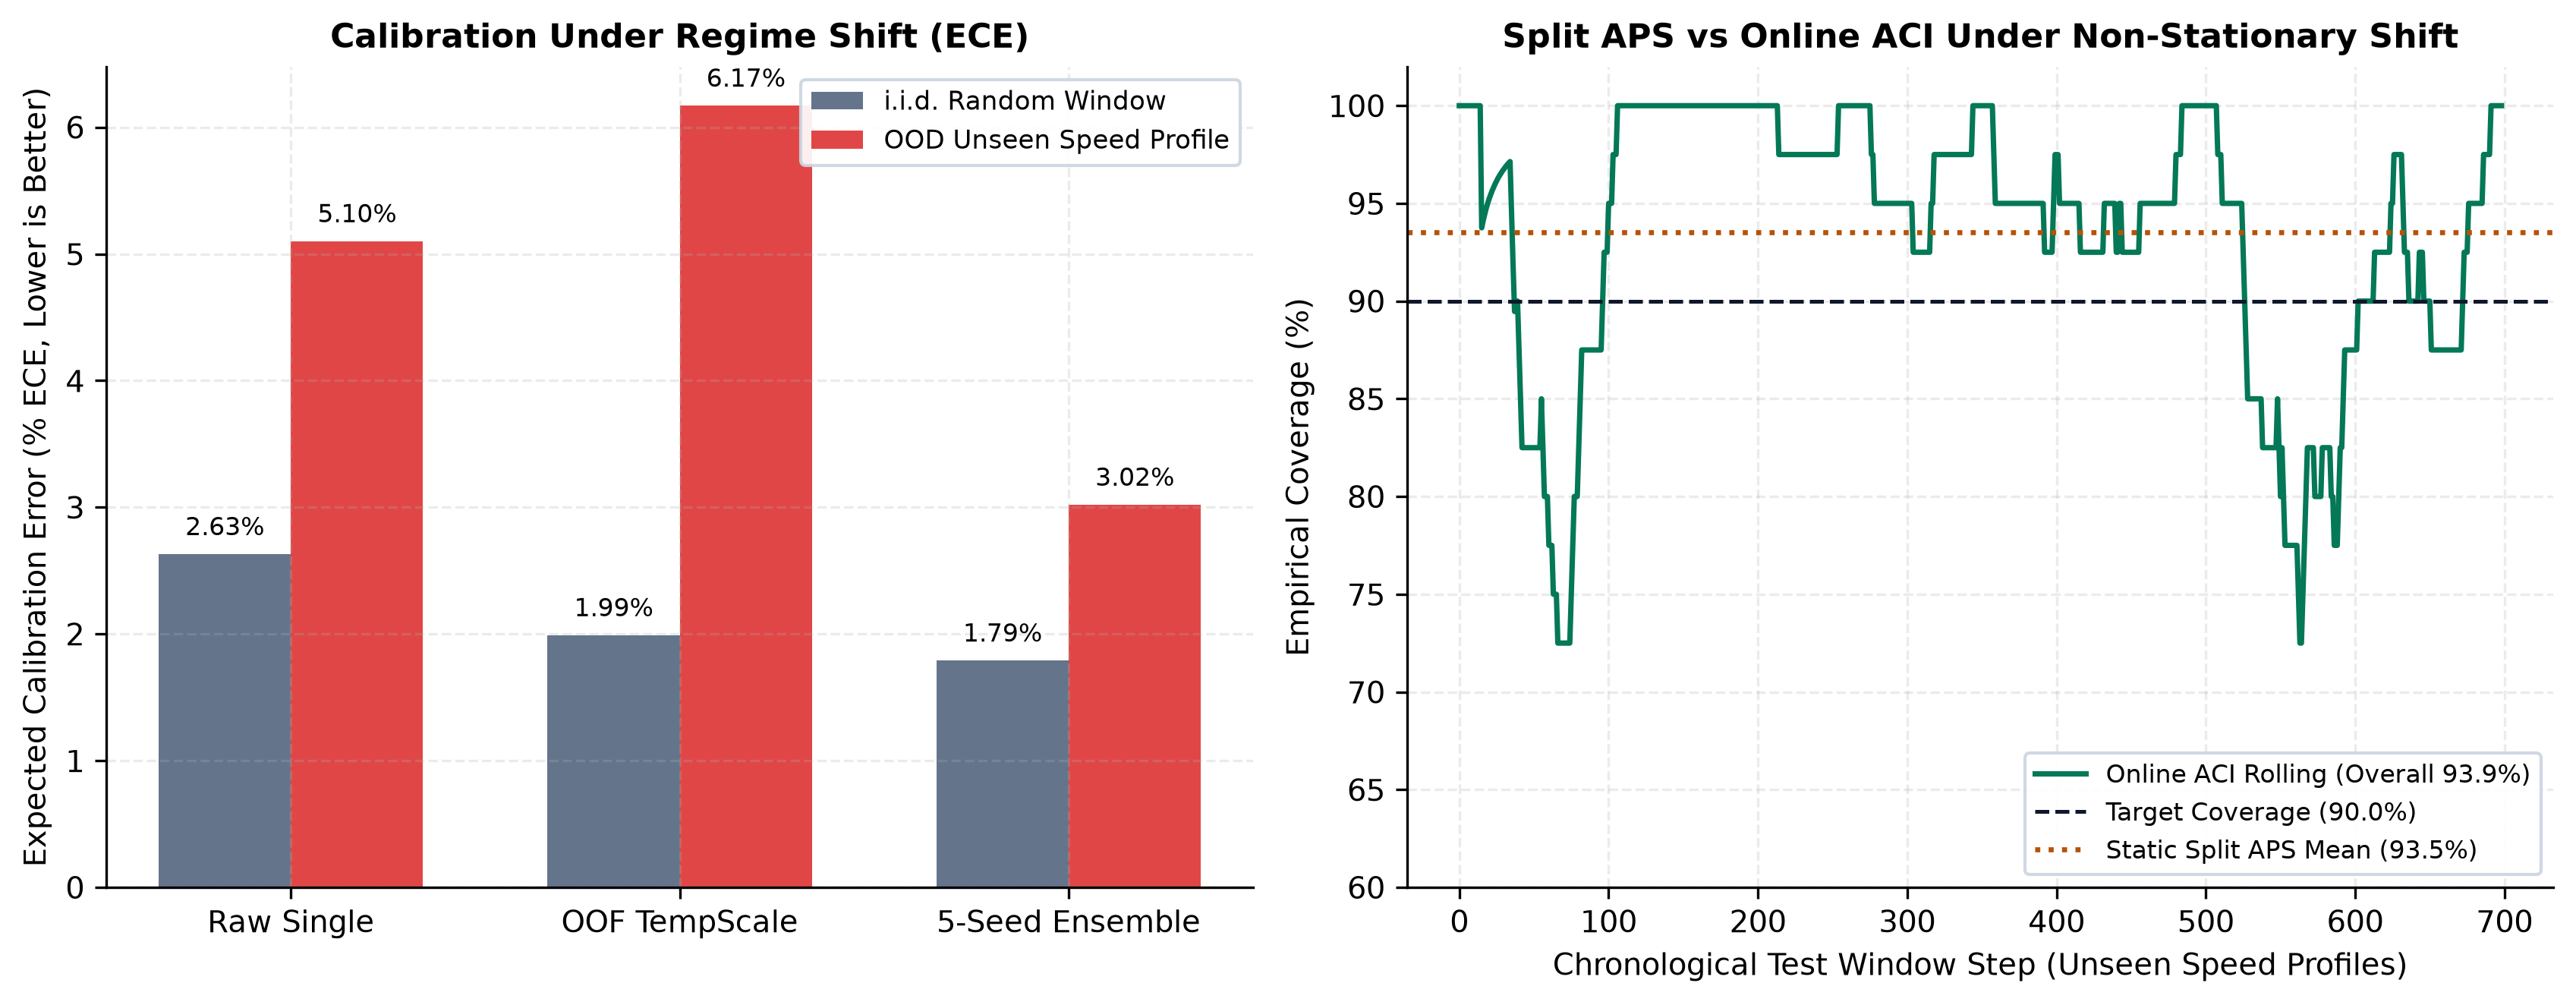
\includegraphics[width=0.96\textwidth]{../assets/fig5_calibration_and_conformal.png}
  \caption{Left: OOD ECE doubles relative to i.i.d.\ splits; ID-tuned temperature scaling worsens OOD ECE ($6.17\%$), whereas 5-seed ensembling cuts ECE to $3.02\%$. Right: Online ACI vs.\ Split APS rolling coverage on reversing speed profiles.}
  \label{fig:cal}
\end{figure*}

\begin{figure*}[t]
  \centering
  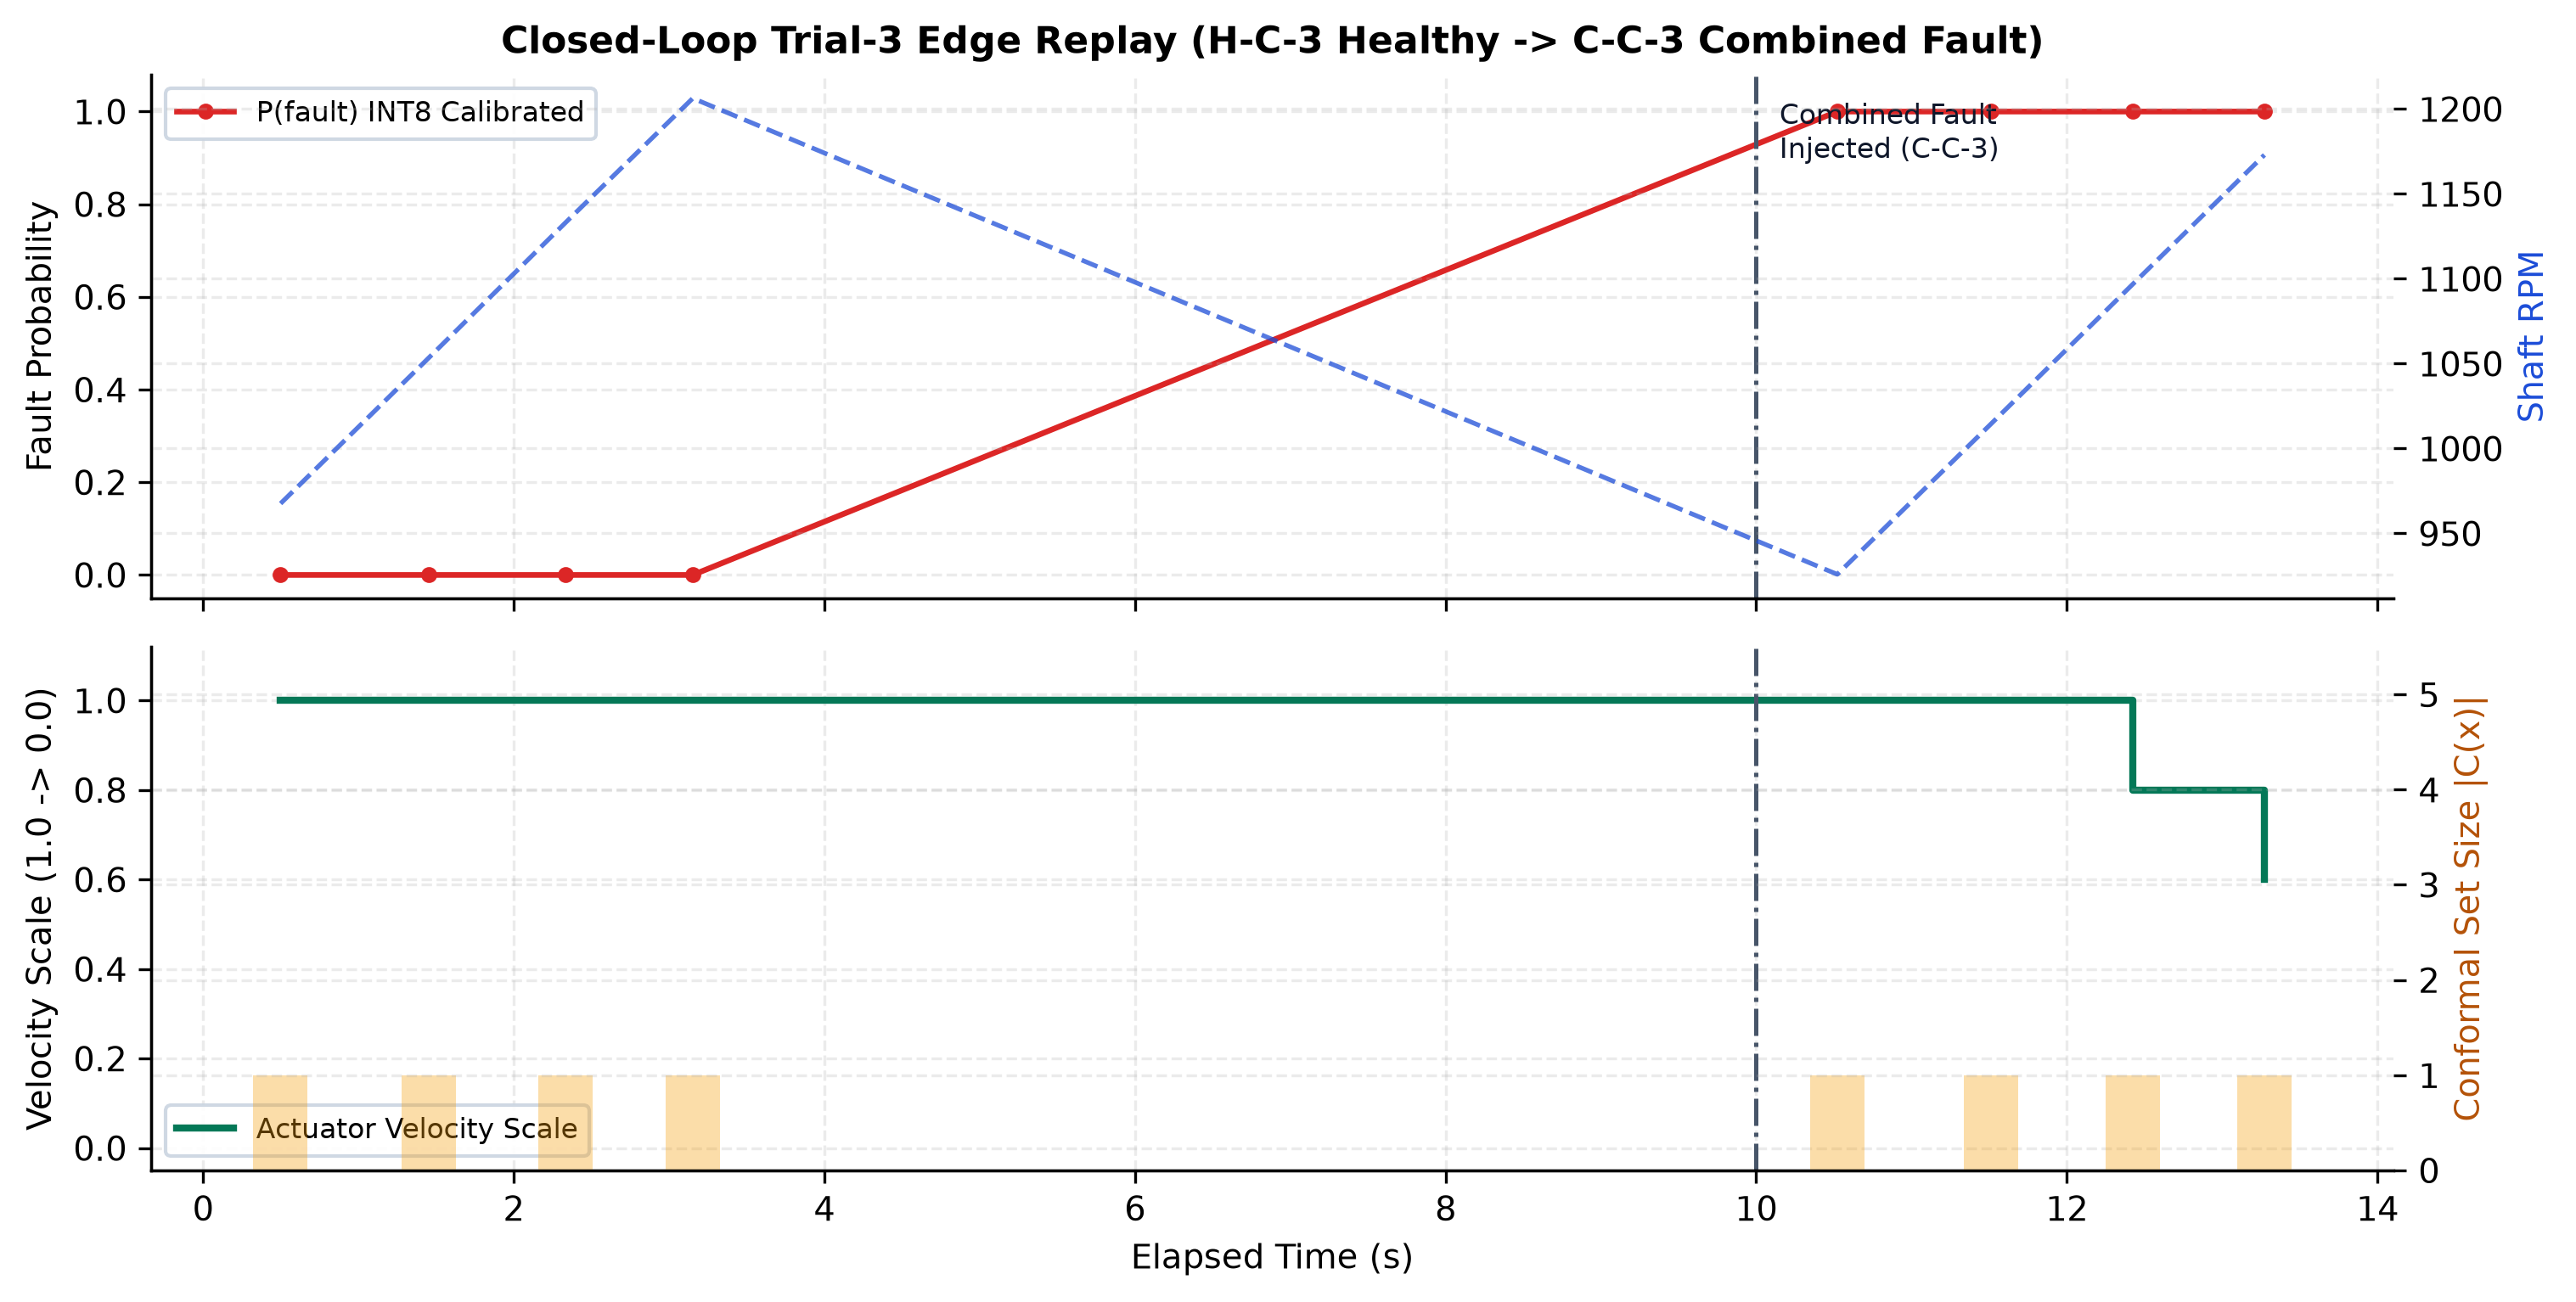
\includegraphics[width=0.92\textwidth]{../assets/fig6_closed_loop_supervisor.png}
  \caption{Closed-loop Trial-3 replay (\texttt{H-C-3} healthy $\rightarrow$ \texttt{C-C-3} combined fault) driving calibrated INT8 probabilities and conformal supervisory control with $0$ false derates.}
  \label{fig:replay}
\end{figure*}

\section{Negative Results and Failure Modes}
Transparently reporting where the pipeline fails defines its operational envelope:
\begin{enumerate}
  \item \textbf{Unseen Fault Severity Wall (CWRU $7/14/21$\,mil):} On \texttt{unseen\_fault\_size}, every model drops sharply (Gain-Sensitive MLP $59.29\%$, 14\,mil fold $33.40\%$; Env CNN $59.63\%$; MRL Env CNN $47.72\%$). Per-diameter physics shifts carrier modulation bandwidth and spectral centroid shape, not mere gain---meaning neither gain invariance nor Matryoshka nesting resolves unseen defect geometries without multi-severity diversity.
  \item \textbf{Split Conformal Breakdown and Finite-Step ACI Lag:} Under CWRU severity shift, Split APS loses exchangeability and drops to $50.16\%$ coverage; Online ACI climbs $+22.88$\,pp to $73.04\%$, still below $90\%$ on short streams because $\gamma=0.05$ step adaptation lags abrupt covariate shifts.
  \item \textbf{ID Temperature Scaling Over-Confidence Under Shift:} Fitting scalar $T$ on proper-train OOF logits slightly worsens uOttawa OOD ECE ($5.10\% \rightarrow 6.17\%$) and increases NLL ($0.4472 \rightarrow 0.7656$).
  \item \textbf{Matryoshka Capacity Knee at $d=8$:} Compressing below $d=16$ raises multi-seed variance ($88.07 \pm 7.66\%$, ECE $0.1777$), identifying $d=16$--$32$ ($20.8$--$22.9\,\text{KB}$) as the reliable floor.
  \item \textbf{CPW Sideband Attenuation:} Pre-whitening slightly degrades uOttawa unseen-speed accuracy ($92.33\%$ vs.\ $92.67\%$), harming low-SNR ball-defect harmonics ($80.44\%$ vs.\ $82.61\%$).
\end{enumerate}

\section{Reproducibility and Conclusion}
Every metric, figure, and INT8 artifact in this report reproduces deterministically from raw \texttt{.mat} files via \texttt{python scripts/reproduce.py} and is cross-checked by \texttt{python scripts/verify\_report\_numbers.py}. Overall, physics-informed envelope-first COT provides the largest generalization gain under non-stationary speed shift ($+7.61$\,pp), nested Matryoshka INT8 compression yields $35.77\,\text{KB}$ CPU models at $92.93\%$ accuracy, and deep ensembles paired with Online ACI expose distribution shifts where static post-hoc calibration fails.

\bibliographystyle{plain}
\bibliography{references}
\end{document}
